\renewcommand{\tmpwidth}{50mm}
\setlength{\tabcolsep}{2pt}
\begin{figure*}[!ht]
    \centering
    \begin{tabular}{c c c}

   
    BigGAN-deep (FID=$6.95$) & VQVAE-2$^\dagger$ (FID=$31$) & \model  (FID=\bestfid) \\
    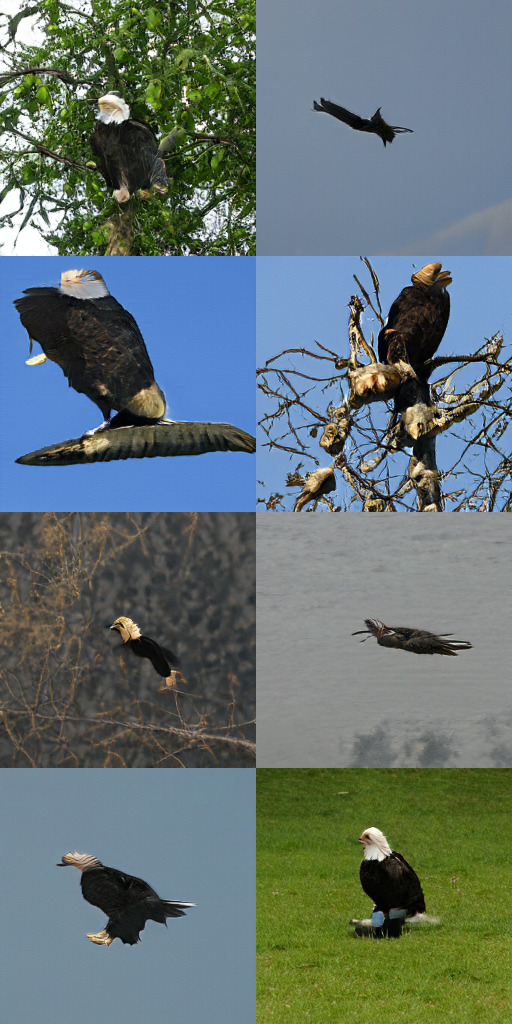
\includegraphics[ width=\tmpwidth]{figures/supp_cc/22_bald-eagle_biggan.jpg} & 
    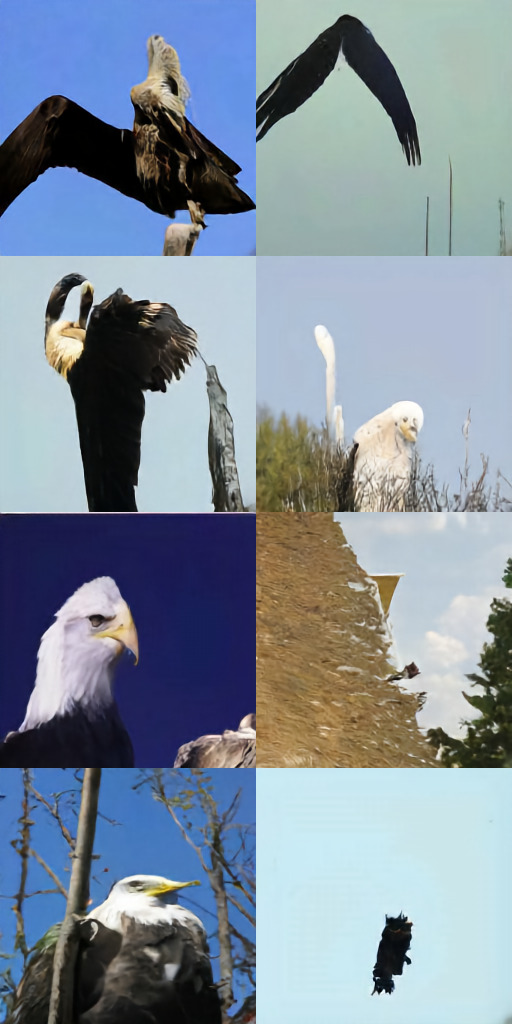
\includegraphics[ width=\tmpwidth]{figures/supp_cc/22_bald-eagle_vqvae2.jpg}& 
    % 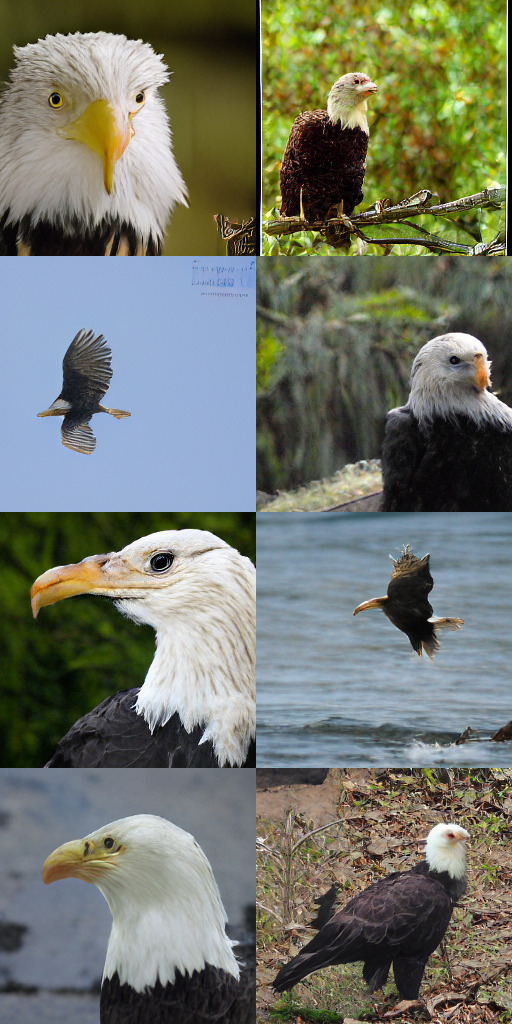
\includegraphics[ width=\tmpwidth]{figures/supp_cc/22_bald-eagle_vqgan.jpg} & \ 
    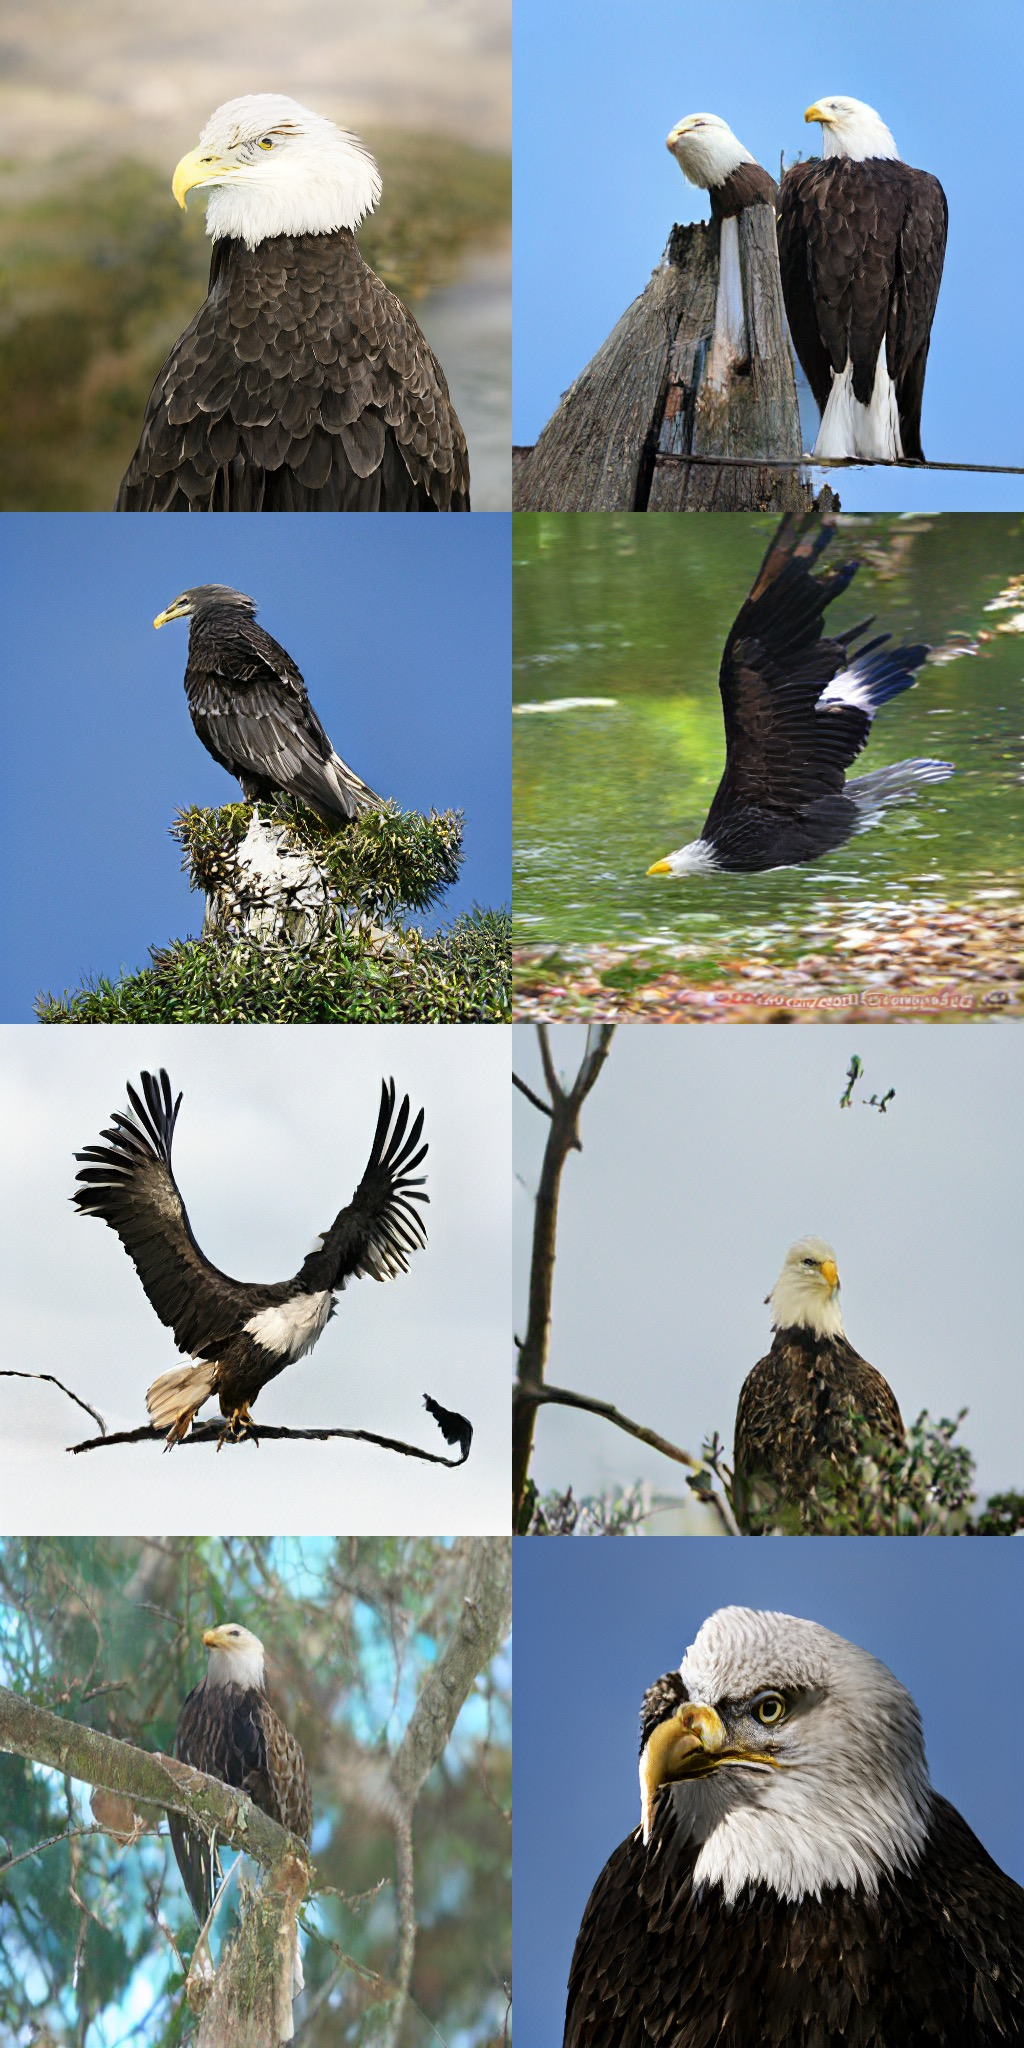
\includegraphics[ width=\tmpwidth]{figures/supp_cc/22_bald-eagle_ours.jpeg} \\ 
       
    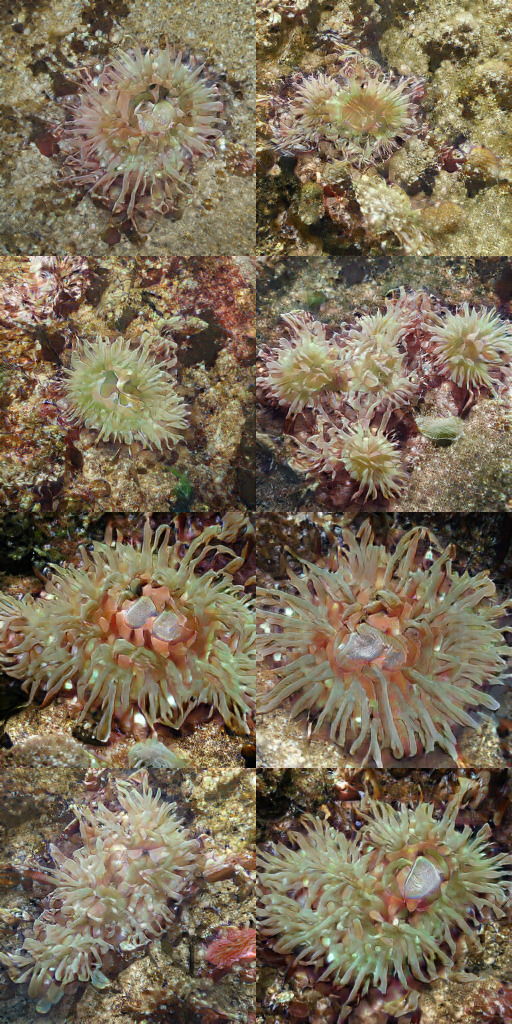
\includegraphics[ width=\tmpwidth]{figures/supp_cc/108_anemone_biggan.jpg} & \
    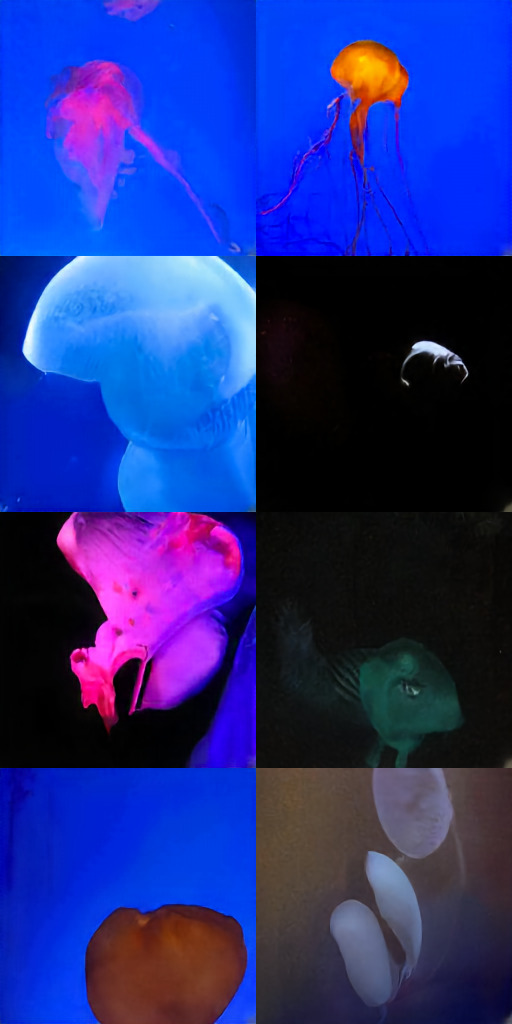
\includegraphics[ width=\tmpwidth]{figures/supp_cc/108_anemone_vqvae2.jpg}& \
    % 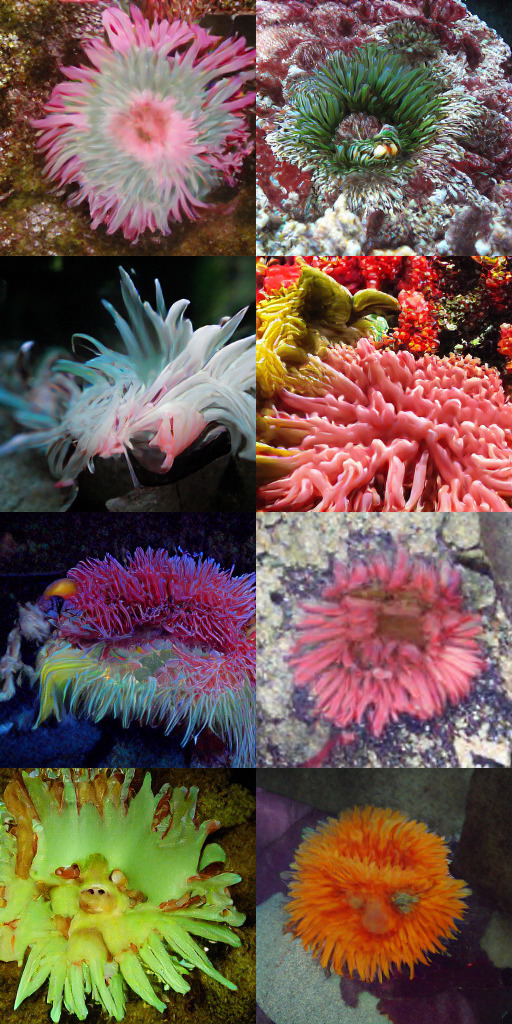
\includegraphics[ width=\tmpwidth]{figures/supp_cc/108_anemone_vqgan.jpg} & \ 
    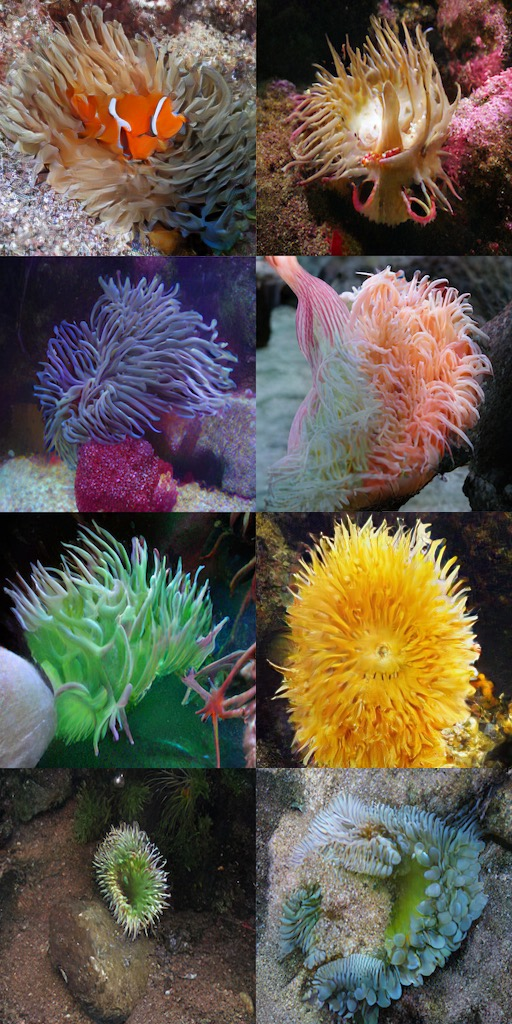
\includegraphics[ width=\tmpwidth]{figures/supp_cc/108_anemone_ours.jpeg} \\ 
    
    
    \end{tabular}
    \caption{\textbf{更多多样性比较}BigGAN-deep（截断值 1.0）、VQVAE-2\cite{Razavi19vqvae2} 和我们提出的方法 \model  在 ImageNet 上的比较。$^\dagger$ 表示从论文中提取的样本。}
    \vspace{-6mm}
    \label{fig:supp_cc_diversity}
\end{figure*}
    
\begin{figure*}[!ht]
    \centering
    \begin{tabular}{c c c}
    
    BigGAN-deep (FID=$6.95$) & VQVAE-2 (FID=$31$) & \model  (FID=\bestfid) \\
    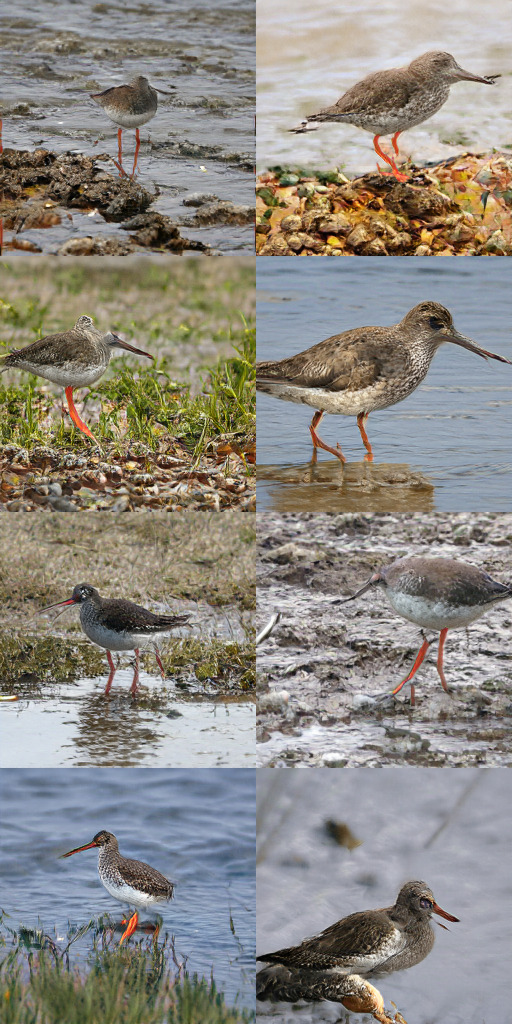
\includegraphics[ width=\tmpwidth]{figures/supp_cc/141_redshank_biggan.jpg} & \
    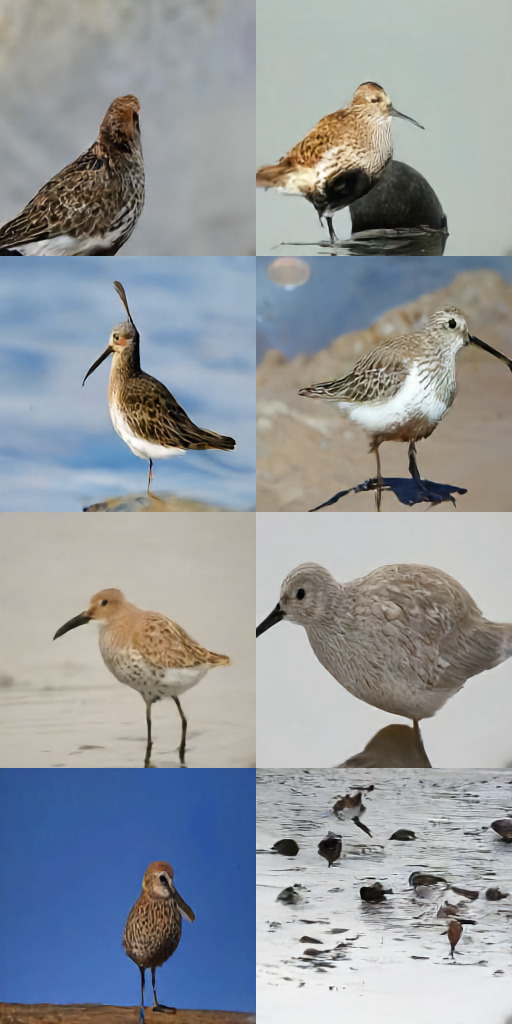
\includegraphics[ width=\tmpwidth]{figures/supp_cc/141_redshank_vqvae2.jpg}& \
    % 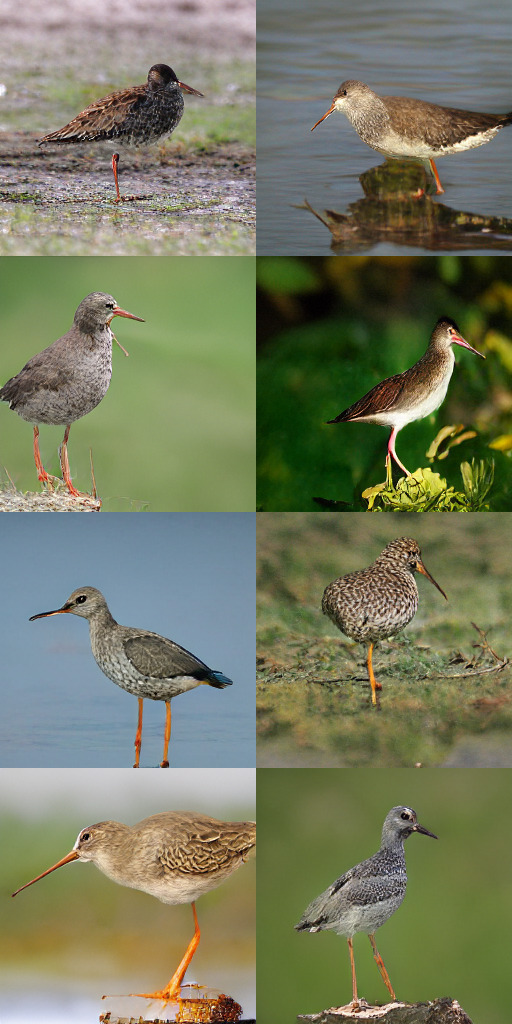
\includegraphics[ width=\tmpwidth]{figures/supp_cc/141_redshank_vqgan.jpg} & \ 
    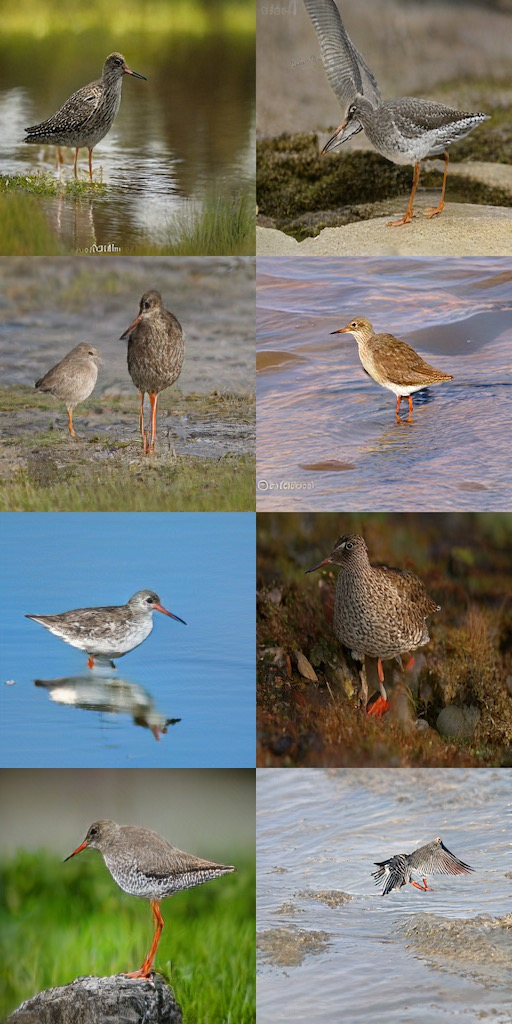
\includegraphics[ width=\tmpwidth]{figures/supp_cc/141_redshank_ours.jpeg} \\ 
    
    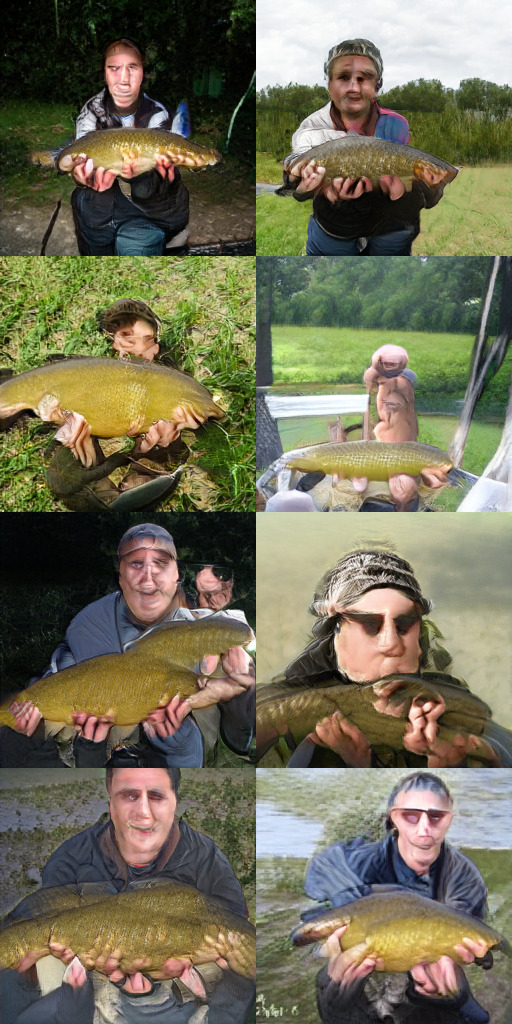
\includegraphics[ width=\tmpwidth]{figures/supp_cc/0_tench_biggan.jpg} & \
    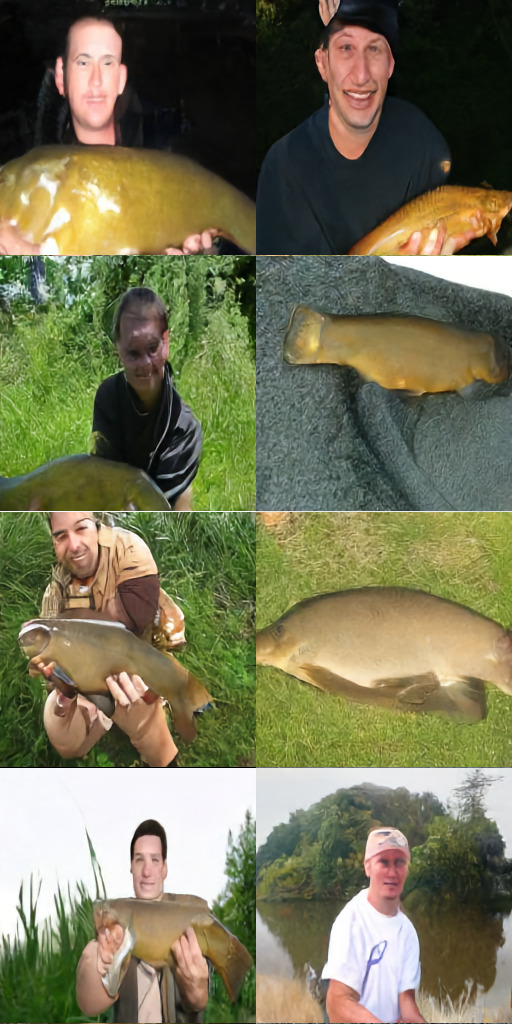
\includegraphics[ width=\tmpwidth]{figures/supp_cc/0_tench_vqvae2.jpg}& \
    % 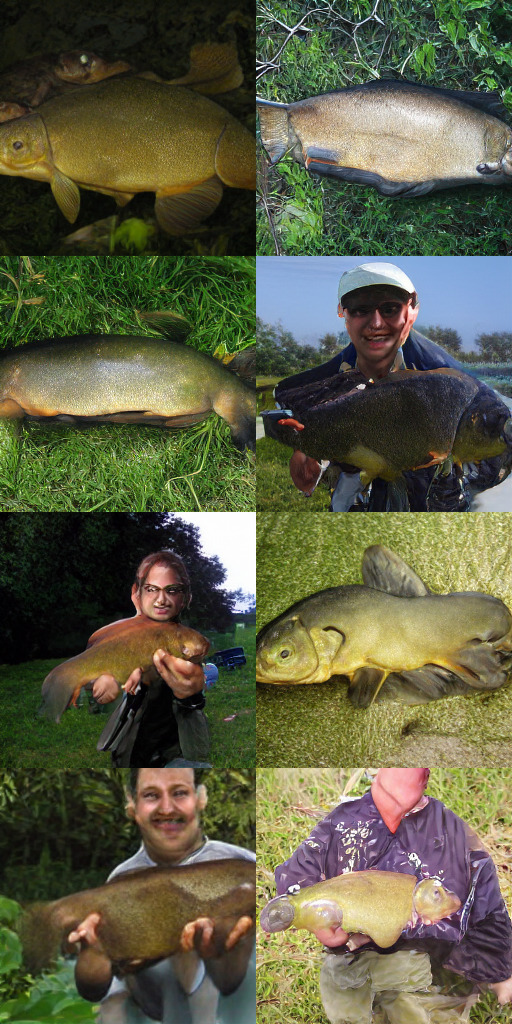
\includegraphics[ width=\tmpwidth]{figures/supp_cc/0_tench_vqgan.jpg} & \ 
    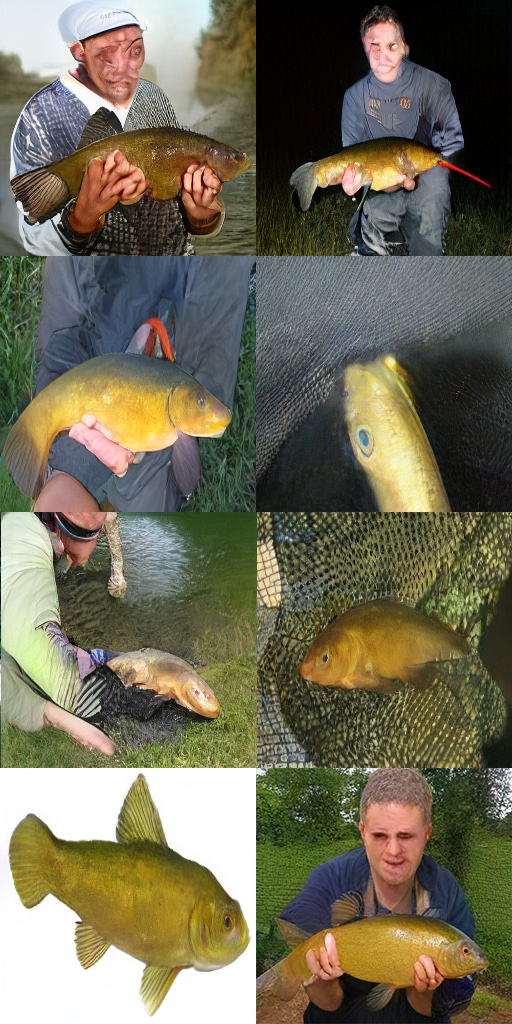
\includegraphics[ width=\tmpwidth]{figures/supp_cc/0_tench_ours.jpeg} \\ 
     
    \end{tabular}
    \caption{\textbf{更多多样性比较}BigGAN-deep（截断值 1.0）、VQVAE-2\cite{Razavi19vqvae2} 和我们提出的方法 \model  在 ImageNet 上的比较。$^\dagger$ 表示从论文中提取的样本。}
    \vspace{-6mm}
    \label{fig:supp_cc_diversity_1}
\end{figure*}   



\begin{figure*}[!ht]
    \centering
    \begin{tabular}{c c c}
    BigGAN-deep (FID=$6.95$) & VQVAE-2 (FID=$31$) & \model  (FID=\bestfid)  \\
    
    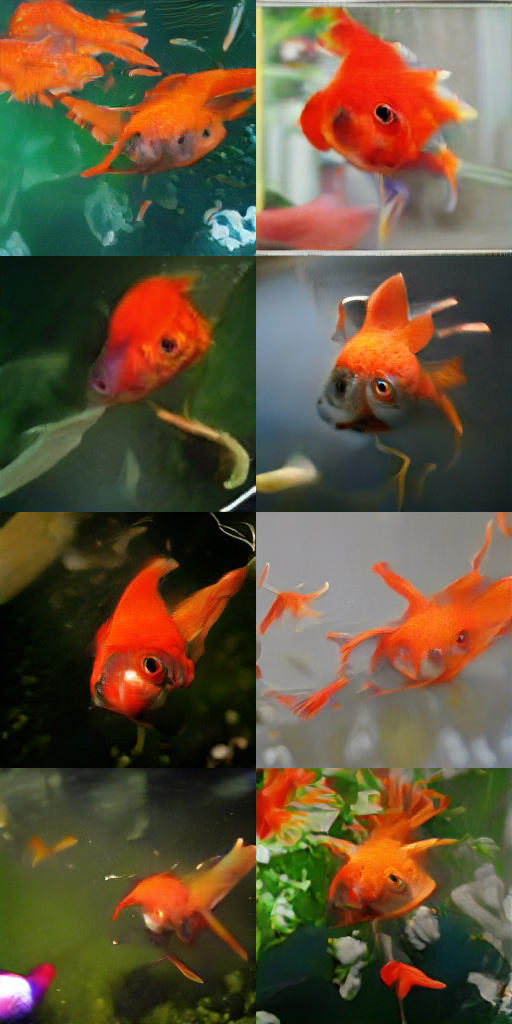
\includegraphics[ width=\tmpwidth]{figures/supp_cc/1_goldfish_biggan.jpg} & \
    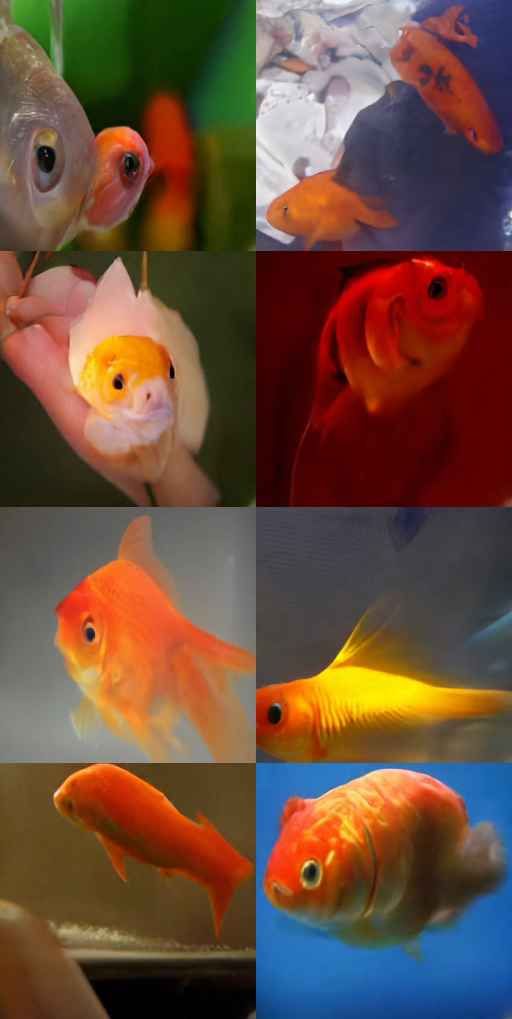
\includegraphics[ width=\tmpwidth]{figures/supp_cc/1_goldfish_vqvae2.jpg}& \
    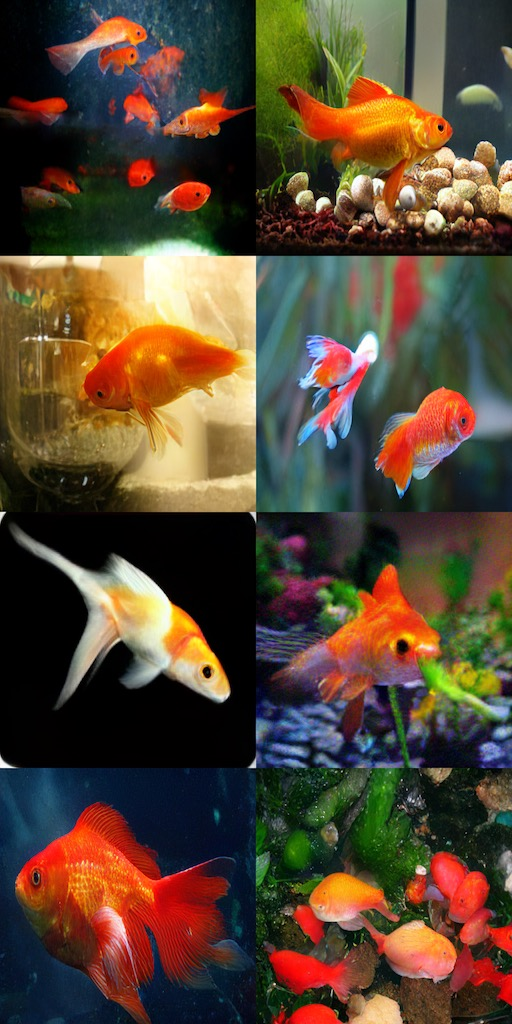
\includegraphics[ width=\tmpwidth]{figures/supp_cc/1_goldfish_ours.jpeg} \\ 
    
    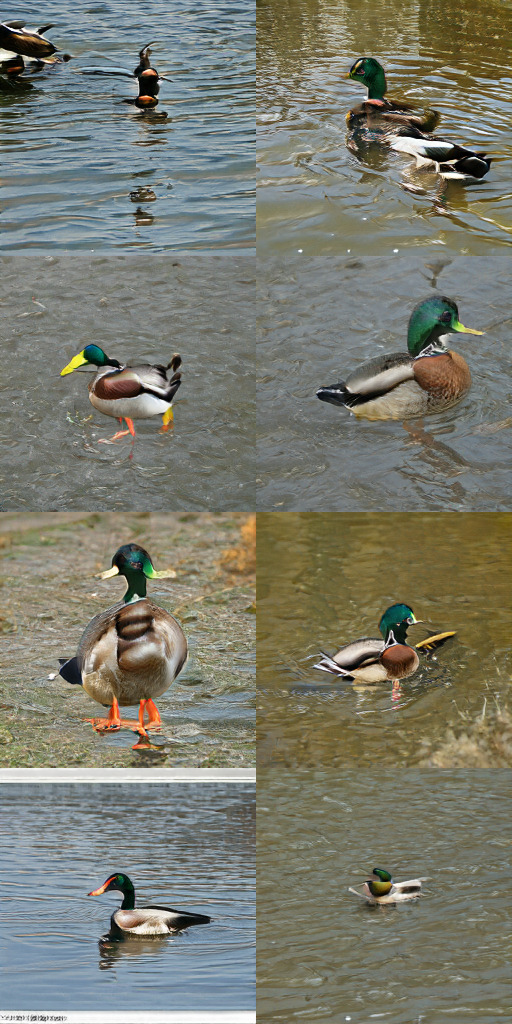
\includegraphics[ width=\tmpwidth]{figures/supp_cc/97_drake_biggan.jpg} & \
    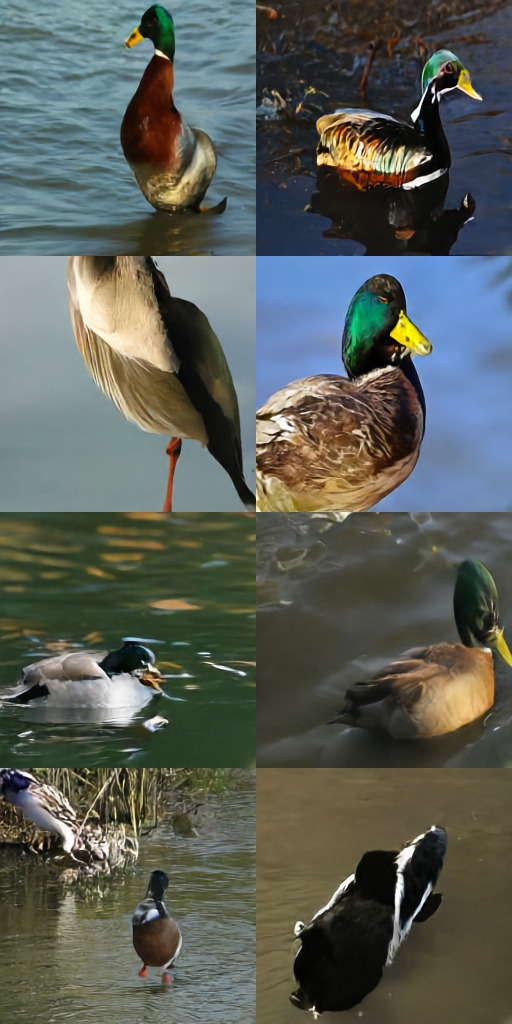
\includegraphics[ width=\tmpwidth]{figures/supp_cc/97_drake_vqvae2.jpg}& \
    % 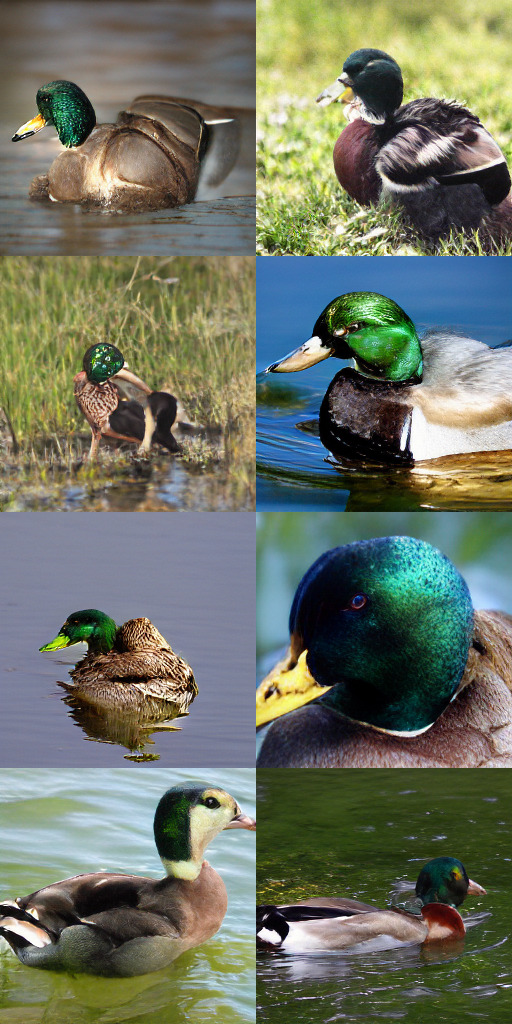
\includegraphics[ width=\tmpwidth]{figures/supp_cc/97_drake_vqgan.jpg} & \ 
    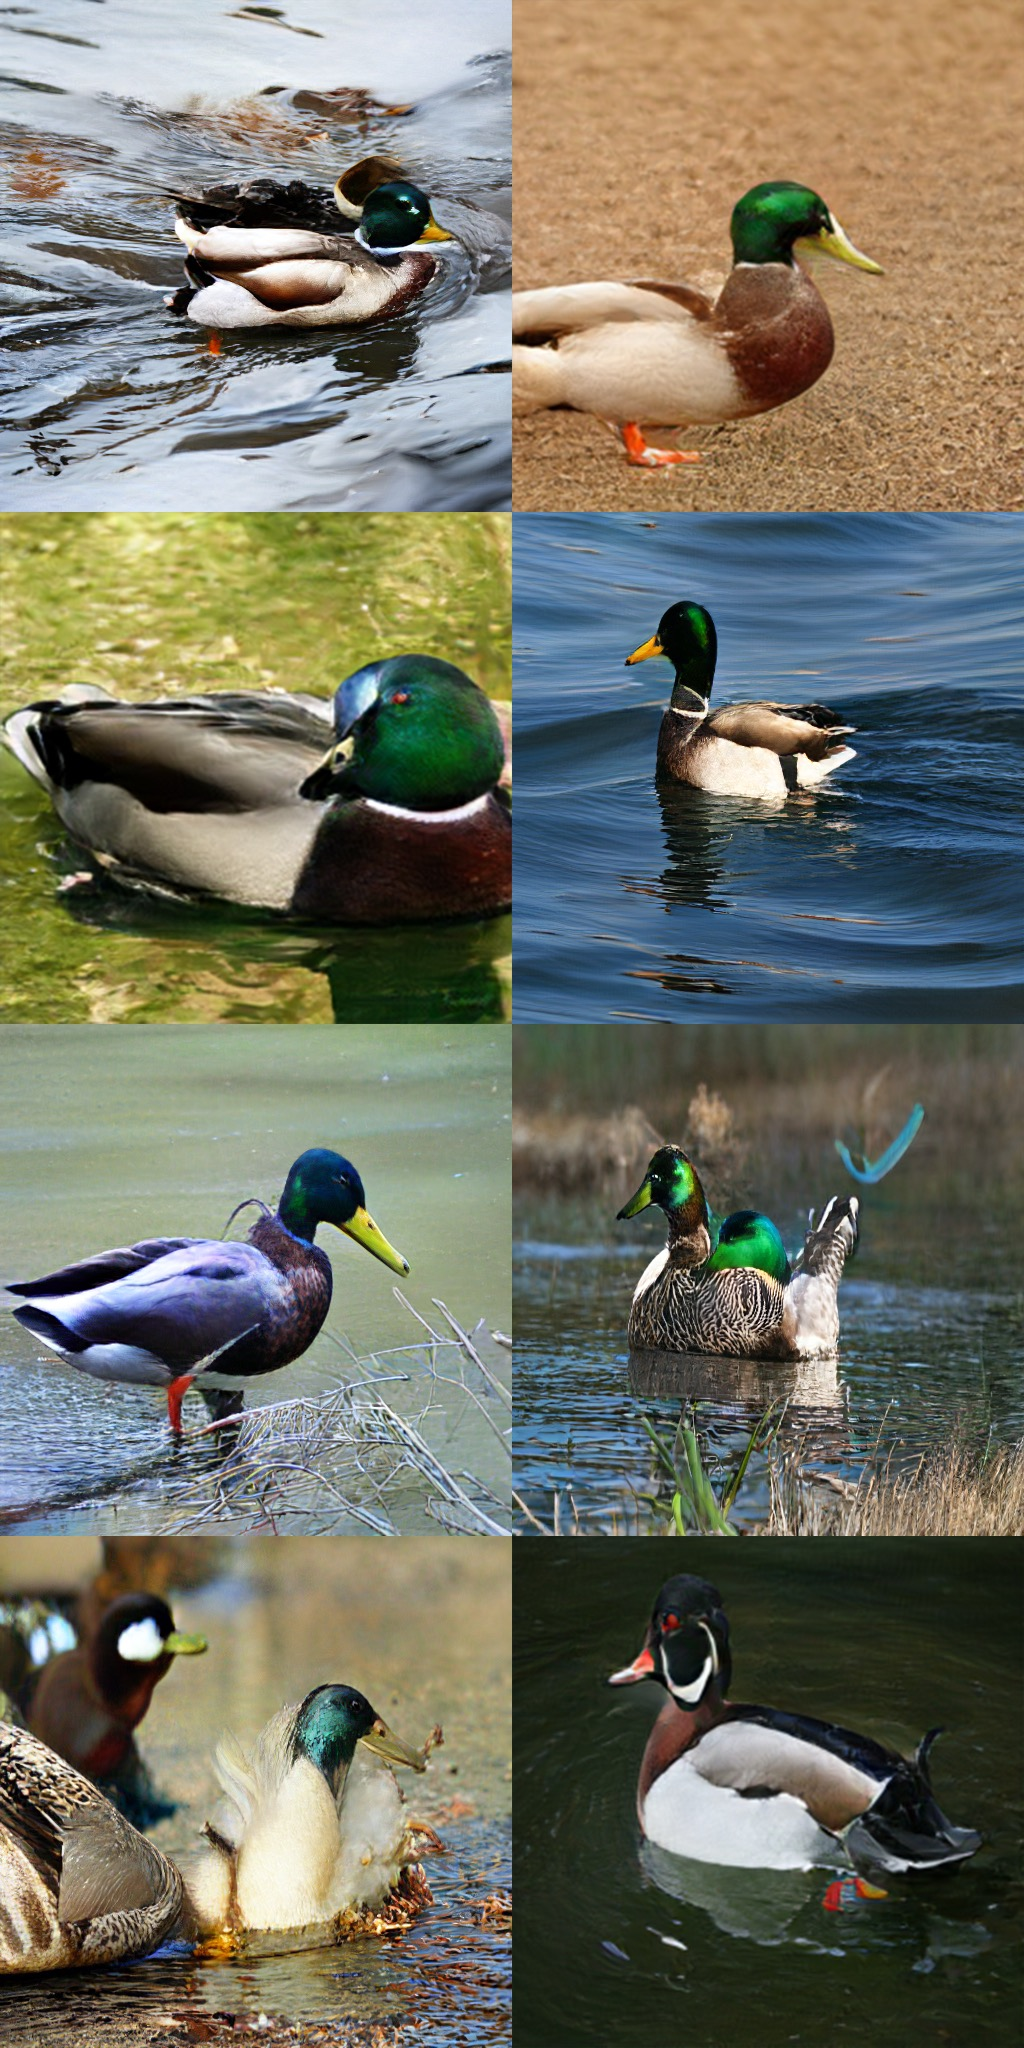
\includegraphics[ width=\tmpwidth]{figures/supp_cc/97_drake_ours.jpeg} \\ 
    
\end{tabular}
    \caption{More Diversity Comparisons among BigGAN-deep with truncation $1.0$, VQVAE-2\cite{Razavi19vqvae2}, and our proposed method \model  on ImageNet. $^\dagger$ represents extracted samples from the paper.}
    \vspace{-6mm}
    \label{fig:supp_cc_diversity_2}
\end{figure*}